\section {GPU architecture}

\acrfull{gpu} is a type of coprocessor designed to work alongside the \acrshort{cpu}, offloading intensive tasks to the coprocessor, accelerating the overall system performance.

Generally speaking, CPUs are low latency, low throughput processors, whereas GPUs are high latency, high throughput processors. A traditional CPU is optimized to execute instructions as fast as possible by reducing \textit{latency} -- the duration from the start of the instruction until the availability of results. To achieve this, CPUs have to implement complex strategies such as speculative branch execution, out-of-order execution, and large memory caches. This architecture works well on workflows, which are sequential by nature, where the execution speed of a single thread has a more noticeable impact on overall execution time.

In contrast, a GPU focuses on hiding the latency instead of reducing it by focusing more on \textit{throughput} -- the amount of work completed per unit of time. The workflows GPUs are most suited for are abundant in parallelism, for example, image processing or matrix multiplication. This assumption drives the design of a GPU to sacrifice the execution speed of a single thread in favor of the sheer amount of processing cores to increase throughput. The difference in design philosophies can be seen in Figure \ref{figure:cpu-vs-gpu}.

Thus, even if the \acrshort{cpu} excels at sequential tasks, the \acrshort{gpu} can outperform the CPU in highly parallel computations, as the sheer number of cores GPU uses compared to CPU execution amortizes the cost of using a slower one \cite{cudaprog}.

\begin{figure}
  \centering
  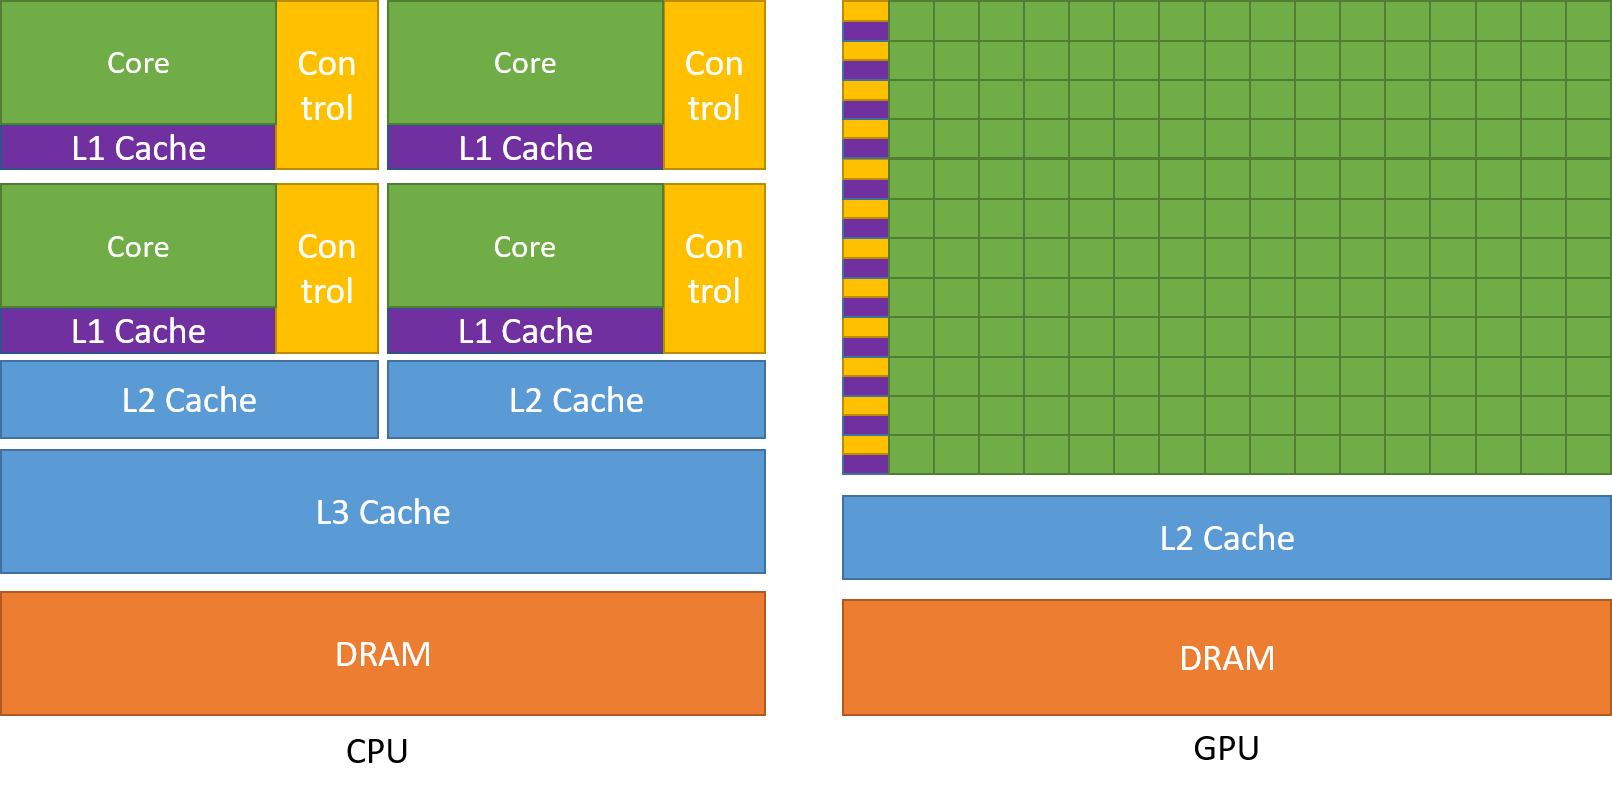
\includegraphics[width=\textwidth]{components/figure/cpu-vs-gpu.png}
  \caption{Comparison of a typical CPU and GPU structure. \cite{cudaprog}}
  \label{figure:cpu-vs-gpu}
\end{figure}

As the staggering performance of a \acrshort{gpu} has not gone unnoticed by the scientific community, work has been done to allow the \acrshort{gpu} to process workloads unrelated to graphics, e.g., linear solvers \cite{cusolver}, or neural networks \cite{cudnn}.

\subsection{Hardware architecture}

As the implementation of both B$^+$Tree and B-Link-Tree is based on CUDA (see Chapter \ref{label:cuda}), we're focusing on NVIDIA \acrshort{gpu} and its architecture in this work. Since the introduction of unified shared architecture with GeForce 8 Series in 2006, a single NVIDIA GPU comprises an array of \textit{streaming multiprocessors} (SM). The power of a single GPU card depends on the number of these streaming multiprocessors, which may vary between models. Each \acrshort{sm} in general have these components:
\begin{itemize}
  \item \textit{Streaming processors}\footnote{Also known as a \textit{CUDA core}}, each containing an arithmetic logic unit (ALU) for integer operations and floating-point unit (FPU) for floating-point operations.
  \item \textit{Register file}, where threads store their local variables. This register file is shared between all threads running in the SM. The number of available registers per thread is defined by architecture.
  \item \textit{Instruction cache}, which caches the instruction without the data for quick fetching.
  \item \textit{Shared memory} used to share data between threads in the same thread block (see Chapter \ref{label:gpu:mem}).
  \item \textit{L1 / Texture cache}, which is used to store local memory of the thread or to serve as a texture cache for image data.
\end{itemize}

Newer architectures include more specialized cores. For example, \textit{tensor cores} in every SP, capable of executing 4x4 matrix multiplication instructions, or \textit{RT cores} in every SM, accelerating raytracing, found in recent Ampere architecture (see Figure \ref{figure:ampere-sm}).

\begin{figure}[H]
  \centering
  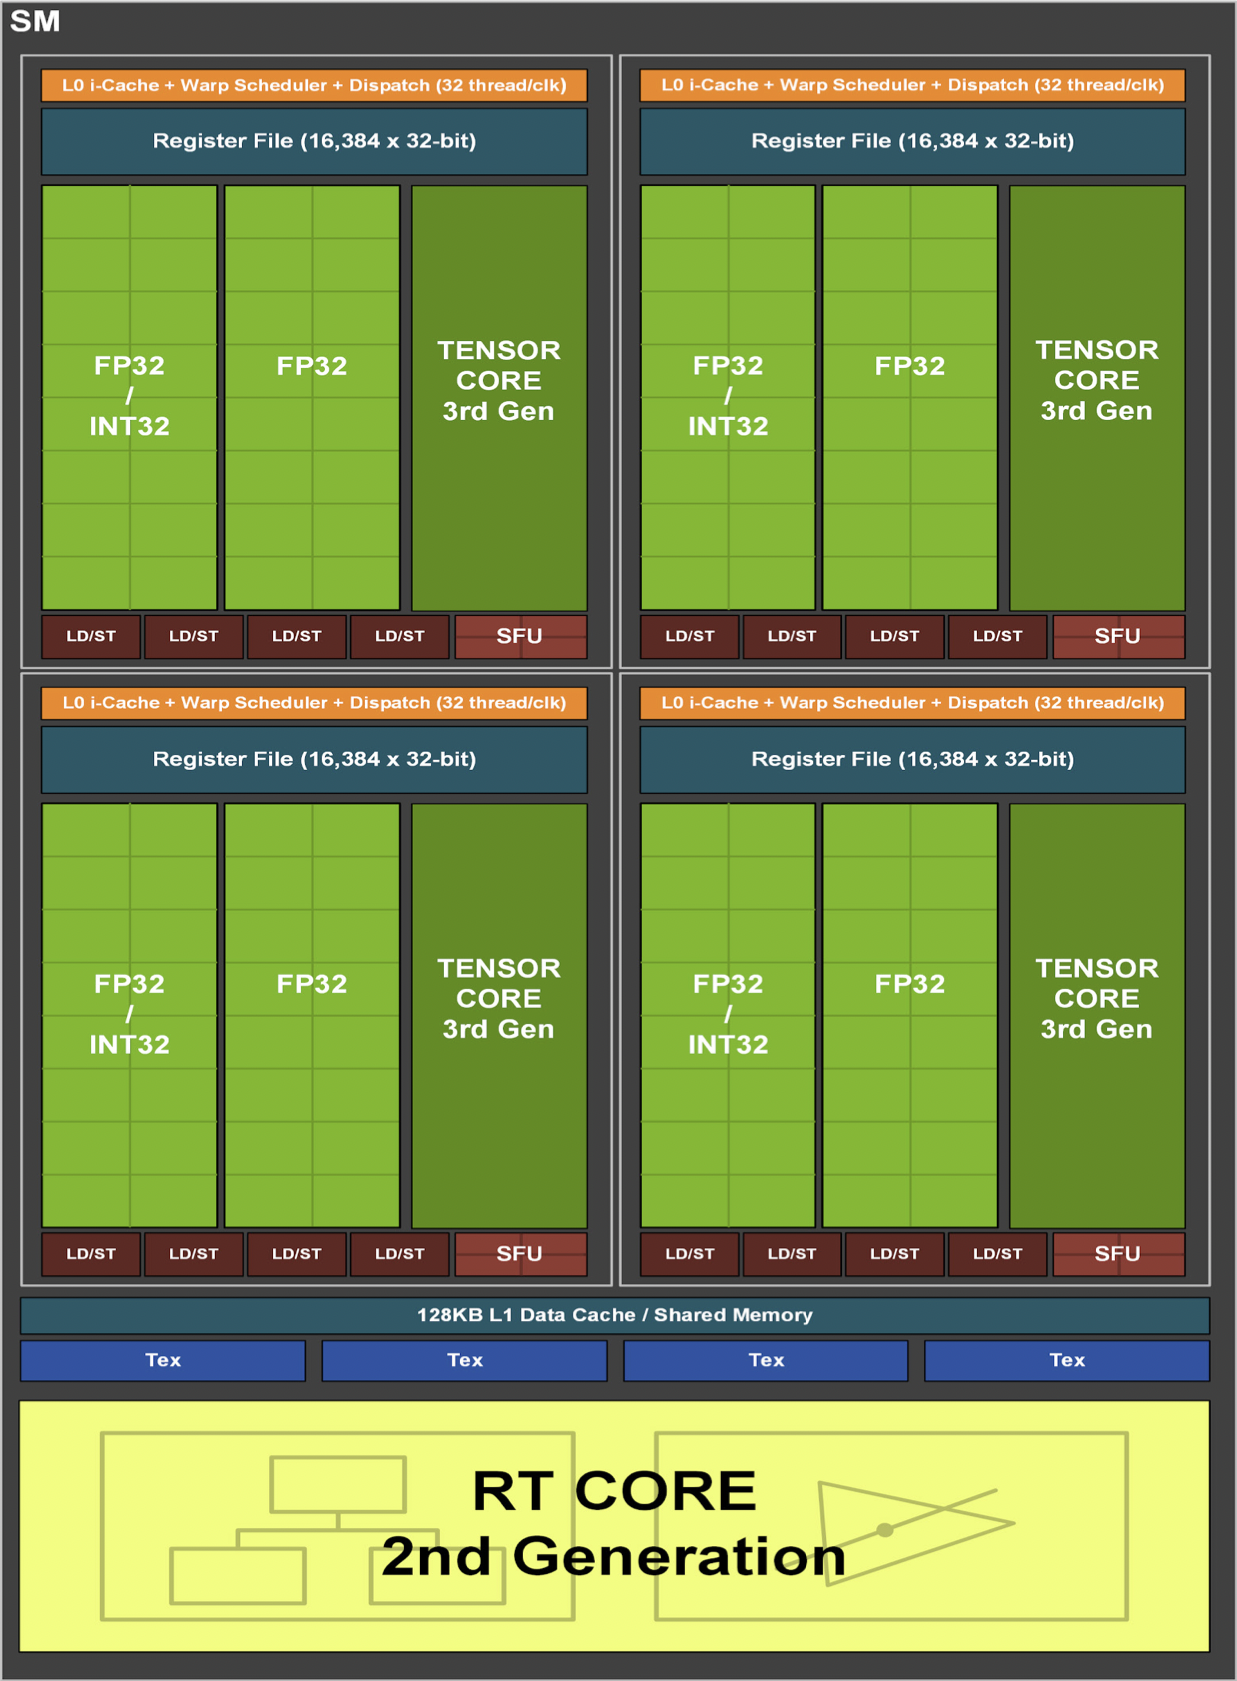
\includegraphics[width=\textwidth]{components/figure/ampere-sm.png}
  \caption{Ampere GA10x Streaming Multiprocessor. \cite{nvidiaampere}}
  \label{figure:ampere-sm}
\end{figure}

\subsection{Memory hiearchy} \label{label:gpu:mem}

The \acrshort{gpu} has its own memory with its memory hierarchy separate from the rest of the system. Every thread has access to its registry and local memory. Local memory is used to store variables for which we do not have space in registers (registry spilling), or we cannot determine if we do have space (like arrays). The registry and the local memory are not directly accessible to the programmer and are managed by the compiler instead.

Each thread also has access to shared memory, which is shared with all threads executing on the same thread block (see Chapter \ref{label:cuda}). As the memory resides on-chip itself, it has higher throughput and lower latency compared to the global memory. It can be considered a user-managed cache, as the application itself takes care of allocation and access to the cache.

Finally, all threads have access to the global memory, available to all threads regardless of the residing multiprocessor. The global memory is the largest memory available on the GPU. But it is also the slowest, as it is stored on a separate chip. Read and writes are done in 32-, 64-, or 128-byte memory transactions \cite{cudaprog}.

Both local and global memory can be routed through L2 and L1 cache. L1 and L2 cache work in a similar manner as in the CPU to speed up memory access. L1 cache level has lower latency than the L2 cache level when accessing, and both of these caches are faster than accessing the memory directly. Thus, to increase memory throughput, it is desirable to store and read data in faster caches than from memory itself -- keeping both cache utilization and hit rate high.

This can be achieved by organizing the memory allocation and access to honor temporal locality, ensuring the duration between the reuse of specific data is as short as possible, and spatial locality, keeping our data access close to each other.

